
\chapter{Conclusion}

\label{ch:conclusion}

This thesis has described three contributions that enable more effective and efficient implementation of high-performance real-time applications on reconfigurable systems.
In this concluding chapter, we recap the key challenges and provide a summary of individual contributions and the significance of each.
Then we will describe the current limitations of this thesis and suggest future research directions.

\section{Summary of Achievements}

An \gls{fpga} contains numerous prefabricated logic and routing resources which allow the functionality and interconnection to be reconfigured.
Many modern \glspl{fpga} have a high level of integration with coarse grained components such as \glspl{dsp}, memory blocks, high-throughput transceivers, peripheral \gls{io}, customisable \gls{ip} blocks and micro-processor cores.
Benefiting from the reconfigurability and abundance of computation resource, \glspl{fpga} have been increasingly adopted to designs with high performance requirements.
\glspl{fpga}' deterministic performance also makes them preferable over \glspl{cpu} and \glspl{gpu} in real-time systems.
However, \glspl{fpga} are restricted in their floating-point computation capability and ability to design in mainstream programming languages.
In addition, the use of \gls{fpga} for real-time applications still lacks focus on high-performance computing capability.
%The effort of linking high-performance computation to the real-time domain is also limited.
This thesis works toward three key areas to address the above mentioned challenges, and makes use of a heterogeneous reconfigurable system to get the best of both \gls{fpga} and \gls{cpu}.

The computation capability of \glspl{fpga} is restricted by the number of logic components available.
Chapter~\ref{ch:precision} discusses how we take advantage of \glspl{fpga}' programmability to fit more floating-point operators to an \gls{fpga} chip.
Instead of using standard IEEE floating-point arithmetic, floating-point operators are implemented in reduced precision which consumes less logic resource and allows higher degree of parallelism, higher clock frequencies and lower \gls{io} bandwidth.
The accuracy loss introduced by reduced precision is compensated by re-computation on \glspl{cpu} using the required output precision.
This chapter proposes a novel data structure and a memory architecture to interface the reduced precision domain on \gls{fpga} and the high precision domain on \gls{cpu}.
As a result, the accuracy of output is the same as an equivalent system fully implemented with high precision data-paths.
We demonstrate that an optimal precision can be chosen that maximises performance by balancing the number of \gls{fpga} data-path and the amount of re-computation on \glspl{cpu}.
The proposed methodology is applied to an image-guided surgical robot application which employs the \gls{pq} process.
The resultant implementation on the reconfigurable system shows a significant speed-up over \gls{cpu}, \gls{gpu} and the same reconfigurable system that has not applied our methodology.

\glspl{fpga}' data-path can be customised and reconfigured for one particular application, so it usually demonstrates better power and energy efficiency compared to \glspl{cpu} and \glspl{gpu}.
However, the power of \glspl{fpga} cannot be neglected as they are increasingly used in the high performance computing domain.
Apart from traditional power saving techniques such as clock gating and dynamic frequency/voltage scaling, Chapter~\ref{ch:adaptation} explores how the unique run-time reconfigurability of \glspl{fpga} could be used as an efficient power saving technique.
The proposed reconfigurable system has two configurations, which allows the \gls{fpga} to run and switch between computation mode and low-power mode.
In computation mode, the \gls{fpga} is clocked at the maximum frequency and all the available resources are utilised to boost performance.
In contrast, for low-power mode, the \gls{fpga} is loaded with a configuration which has the slowest possible clock and uses only the minimal amount of resource.
The proposed run-time reconfiguration approach is applied to a robot localisation application which employs adaptive \gls{smc} methods.
Compared to a non-adaptive and non-run-time-reconfigurable system, the proposed approach reduces idle power by 25-34\% and the overall energy consumption by 17-33\%.
%We optimise the algorithm to make use of the proposed run-time reconfiguration, so the computation workload can be adapted without sacrificing the quality of results.

Although techniques proposed in Chapter~\ref{ch:precision} and Chapter~\ref{ch:adaptation} enhance the computation and energy efficiency of reconfigurable systems,
the design complexity and compilation time of \gls{fpga} applications far exceed that of \glspl{cpu} and \glspl{gpu}, making \glspl{fpga} difficult to be accepted by mainstream application designers.
Chapter~\ref{ch:tool} discusses the programmability challenges, and describes a design flow which extends the \gls{smc} reconfigurable system mentioned in Chapter~\ref{ch:adaptation}.
To make the proposed reconfigurable system more user-friendly, Chapter~\ref{ch:tool} focuses on making the system parametrisable for a wide variety of \gls{smc} applications.
A surrogate modelling-based machine learning algorithm is employed to tune design parameters for improved performance and solution quality. 
The design flow enables efficient mapping of applications to multiple \glspl{fpga}, reduces design space exploration effort, and is capable of producing reconfigurable implementations for a range of SMC applications.
Significant improvement in speed and energy efficiency are achieved over optimised \gls{cpu} and \gls{gpu} implementations.

To conclude, Figure~\ref{fig:intro_organisation_ch6} recaptures the thesis organisation chart in Chapter~\ref{ch:introduction}, and it shows the connections of three contributions that enhance reconfigurable systems for real-time applications.
Unique features of \gls{fpga} technology, in particular customisable precision in Chapter~\ref{ch:precision} and run-time reconfiguration in Chapter~\ref{ch:adaptation}, have been applied to optimise reconfigurable real-time systems.
The long-standing programmability issues of \gls{fpga} has also been addressed by a domain-specific design flow in Chapter~\ref{ch:tool}.
The enhanced computing capability brought by reconfigurable technologies enlarges the set of compute-intensive algorithms that can have realistic applications in daily life.
For example in Chapter~\ref{ch:precision}, we discusses the potential of clinical setting in surgical robots.
The use of customisable precision allows more sophisticated models and higher update rates so that surgeons who use surgical robots are able to response promptly.
In Chapter~\ref{ch:tool}, the design flow reduces the effort of implementing a high-performance air traffic management system.
In addition, the \gls{smc} computation engine provides sufficient computing power in dealing with the growing demand of future air traffic.
An efficient air traffic management system reduces the level of human control, improves fuel consumption, decreases the time of arrival of aircraft, and increases the capacity of airspace.
%Chapter~\ref{ch:tool} shows an unified platform in implementing \gls{smc} applications, also demonstrate flexibility of optimising towards either for speed or solution quality.

\begin{figure}[ht]
\begin{center}
\includegraphics[width=0.7\textwidth]{1_introduction/figures/organisation}
\end{center}
\caption{Thesis contributions.}
\label{fig:intro_organisation_ch6}
\end{figure}

\section{Future Work}

This section will elaborate on the current limitations of this thesis, and suggest directions in which future research can address them.

%\subsection{Precision Optimisation of Reconfigurable Data-paths}
\subsection{Proximity Query Formulation}

The work in Chapter~\ref{ch:precision} shows the acceleration of \gls{pq} with reconfigurable system.
\gls{pq} has substantial potential in medial surgery which involves human-robot collaborative control.
The proposed reduced precision approach can be extended to cover applications which could not be applied to clinical setting due to complex models and stringent real-time requirements.
One example is image-guided catheterisation as illustrated in Figure~\ref{fig:heart_model}.
To deal with rapid deformation of the heart and the associated blood vessels, it is vitally important to provide the operator of surgical robot online guidance in real time, for which fast and efficient \gls{pq} computation is essential.
The current implementation of \gls{pq} has three limitations that can be improved in the future:
\begin{itemize}
\item \gls{pq} is currently modelled with points and contours, for example in minimal invasive heart surgery, the surgical instrument is described by a cloud of points and the aorta vessel is modelled by a series of contours.
The data structure and memory buffer are designed specifically for this point-contour model. %which limits the availability in various kinds of applications.
In the future, the \gls{pq} formulation can be extended to point-point model to maximise the flexibility.
Such an extended model will increase the computation requirement, thus a faster reconfigurable system is necessary.
\item The proposed heterogeneous reconfigurable system connects \glspl{fpga} and \glspl{cpu} via the PCI Express bus.
Data accessed by \glspl{fpga} have to be copied from the main memory hosted by \glspl{cpu}, and vice versa.
The performance of such decoupled heterogeneous architecture is restricted by high latency and limited bandwidth.
In the future, we can investigate closely-coupled platform where \gls{cpu} and \gls{fpga} fabric lie in the same board or even the same chip.
One example is \gls{soc}-\gls{fpga} introduced by Altera~\cite{alterasoc} and Xilinx~\cite{xilinxzynq}.
Figure~\ref{fig:altera_soc} shows the block diagram of an Altera \gls{soc}-\gls{fpga} which integrates an ARM-based hard processor, input/output peripherals, memory interfaces and FPGA fabric.
\gls{amba} provides high throughput interconnect between \glspl{cpu} and \glspl{fpga}.
This closely-coupled platform follows the topologies described in Figure~\ref{fig:het_arch}.
The \glspl{fpga} partition acts as a deterministic real-time co-processor which connects to peripherals.
The ARM processor runs a \gls{rtos} to serve real-time requests in software.
\item At present, the run-time reconfiguration is done on full chip basis, which means that the entire \gls{fpga} is loaded with a new bit-stream each time it is reconfigured.
On our targeting platform, full chip reconfiguration takes around one second, which precludes its usage in many applications that require fast response time.
In Chapter~\ref{ch:precision}, we try to overcome this drawback by reconfiguring one \gls{fpga} at a time while keeping the remaining \glspl{fpga} operating.
This method needs multiple \gls{fpga} boards to support individual reconfiguration.
It is worth investigating partial reconfiguration technique, where only a subset of the design is changed at run-time.
To do this, the design is partitioned into two regions.
The critical sections of the data-path, such as those having reduced precision arithmetic, are run-time reconfigurable.
The remaining parts, such as PCI Express interface and memory controller, can be kept static.
Instead of disabling an entire \gls{fpga} board for reconfiguration, the proposed scheme still allows some data-paths to be functioning during reconfiguration.
%These applications, such as the real-time \gls{pq} between a robotic device and a rapidly deforming anatomy, will help us to evaluate the impact of run-time reconfiguration on various data sets.
\end{itemize}

\begin{figure}[t!]
\centering
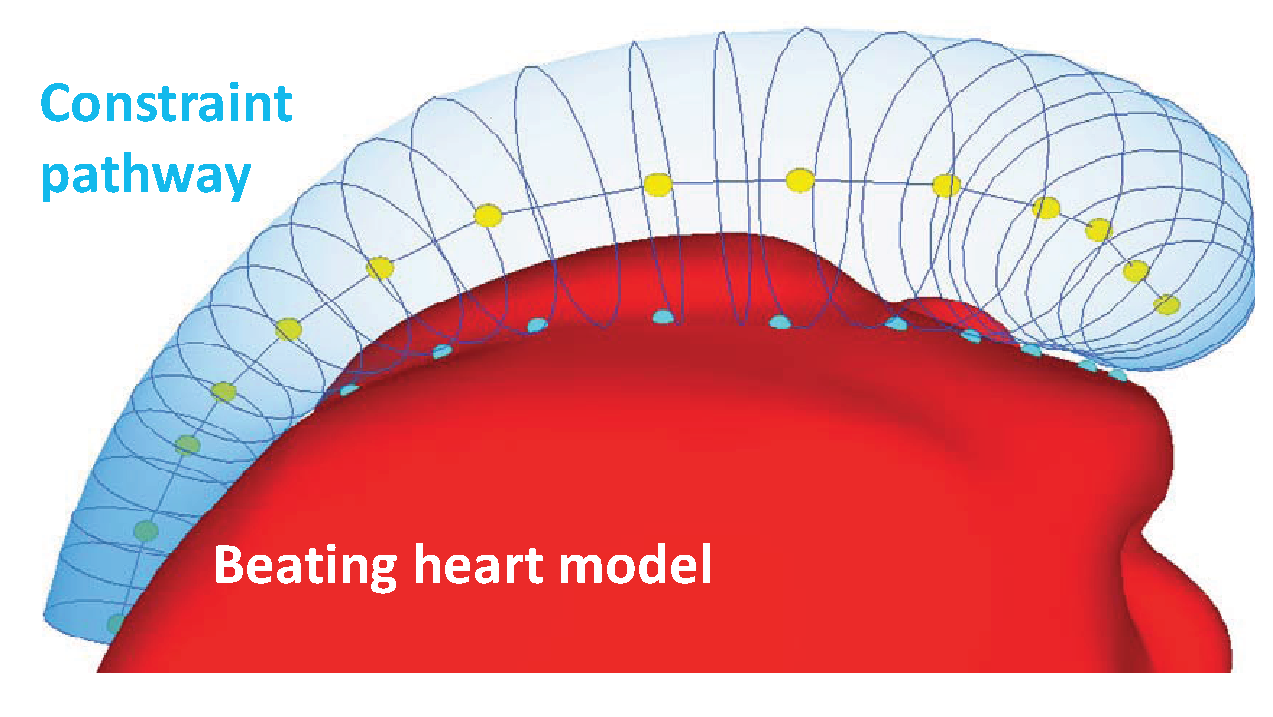
\includegraphics[width=0.6\textwidth]{6_conclusion/figures/heart_model}
\caption{Image-guided catheterisation: Perform PQ based on a beating heart model, where light blue bubbles represent the control points registered on the surface and yellow spheres indicate the control points forming the centre line of the pathway~\cite{kwok13}.}
\label{fig:heart_model}
\end{figure}

\begin{figure}[t!]
\centering
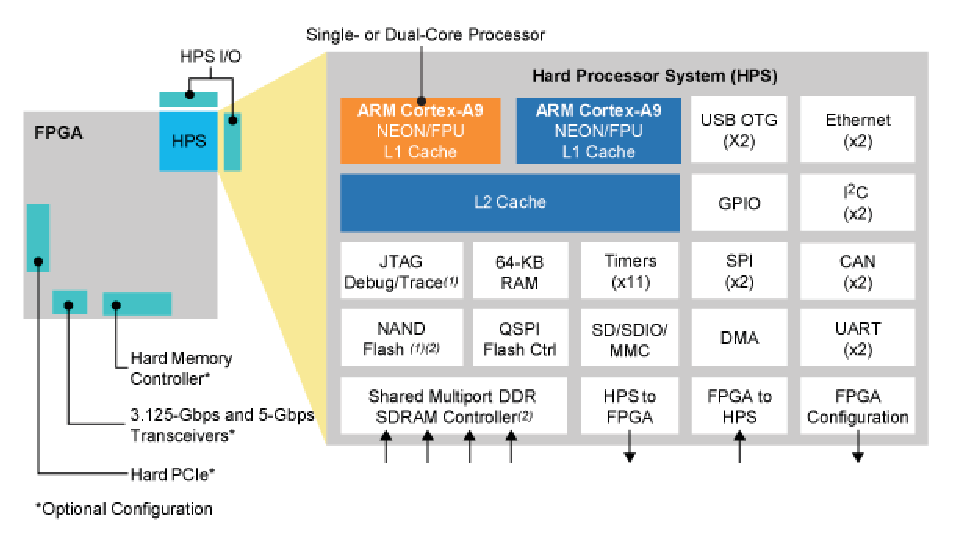
\includegraphics[width=0.8\textwidth]{6_conclusion/figures/altera_soc}
\caption{Altera SOC which integrates an ARM-based hard processor, peripherals, memory interfaces and FPGA fabric~\cite{alterasoc_hps}.}
\label{fig:altera_soc}
\end{figure}

%\subsection{Run-time Adaptation of System Configuration}

%Heterogeneous reconfigurable systems will be developed for various particle filters that are more compute-intensive and have more stringent real-time requirements than the ones described above.
%Air traffic management~\cite{chau13acm} and traffic estimation~\cite{mihaylova07} are example applications that can substantially benefit from the proposed approach in meeting current and future requirements.
%Further work will also be required to automate the optimisation of designs targeting heterogeneous reconfigurable systems.

\subsection{Adaptive Sequential Monte Carlo Methods}

%The work presented in Chapter~\ref{ch:adaptation} can also be benefited by partial run-time reconfiguration.
In Chapter~\ref{ch:adaptation}, the proposed reconfigurable system switches between computation mode and low-power mode.
Currently, the system performance is restricted by full-chip reconfiguration, 
as it consumes time and energy, shortens idle time, and keeps applications which require fast response time away from this system.
In fact, PCI Express interface and memory controller should be in place for both configurations as these components are crucial to maintain functionality.
To reduce reconfiguration overhead, these components need not to be reconfigured.

Apart from partial reconfiguration, the fixed computation interval of real-time system can be exploited by other power saving techniques as summarised in Figure~\ref{fig:partial_scheme}:

\begin{figure}[t!]
\centering
\includegraphics[width=0.6\textwidth]{6_conclusion/figures/partial_scheme}
\caption{Different schemes to put FPGA to sleep.}
\label{fig:partial_scheme}
\end{figure}

\begin{itemize}
\item \gls{dfs}: Instead of the ``best-effort'' approach which finishes the computation as quickly as possible (Figure~\ref{fig:adaptive_scheme_1}), we can use a ``just-in-time'' approach (Figure~\ref{fig:adaptive_scheme_2}) which lowers the clock speed to an extent that the system could finish just within the real-time interval.
To enable this approach, effective and efficient real-time scheduling should be studied to guarantee meeting real-time requirement.
\item Clock gating: This is a common power optimisation technique employed in both \gls{asic} and \gls{fpga} designs to eliminate unnecessary switching activity and thus dynamic power consumption.
To enable clock gating, designers need to add additional gating components to the \gls{rtl} code.
The added components disable unnecessarily active sequential elements which need not to switch states.
In \glspl{asic}, the clock nets that distribute the clocks to all sequential elements are built specifically for each device.
The clock nets can be added with any gating component to gate particular groups of clocks, and the delays introduced by these gating components are specifically handled.
In \glspl{fpga}, the clock nets are fixed because dedicated nets and buffers are responsible for distributing the clocks to all logic elements.
To disable a clock net without introducing glitches, or to switch a clock net between two clock frequencies, designer needs to allocate global clock buffers carefully.
Static circuit and gated circuit can be assigned to different global clock buffers, but the number of global clock buffers are limited and using too many of them can potentially draw more power than that saved by clock gating.
%It is not possible to do the arbitrary gating that is possible in \glspl{asic}.
%In addition, adding gating components and determining portions of gated circuit require intimate knowledge of the design and numerous changes to the \gls{rtl}.
%For example, if a clock is gated using a \gls{lut}, the clock needs to leave the clock network and be routed using general routing resources to a \gls{lut}, and then be routed back to the desired clock. 
%The \glspl{lut} used for clock gating can introduce glitch and the extra routing can make the clock arrive later than any clock that stays on the clock tree.
\end{itemize}

\setcounter{subfigure}{0}
\begin{figure}[t!]
\centering
\subfigure[]{
	\includegraphics[width=0.48\textwidth]{6_conclusion/figures/adaptive_scheme_1}
	\label{fig:adaptive_scheme_1}
}
\subfigure[]{
	\includegraphics[width=0.48\textwidth]{6_conclusion/figures/adaptive_scheme_2}
	\label{fig:adaptive_scheme_2}
}
\caption{(a) Best-effort adaptive scheme described in Chapter~\ref{ch:adaptation}; (b) Just-in-time adaptive scheme.}
\end{figure}

As mentioned earlier in this chapter, the proposed heterogeneous reconfigurable system consists of \glspl{fpga} and \glspl{cpu} which are not closely coupled.
In Chapter \ref{ch:adaptation}, particle data are transferred frequently between \glspl{fpga} fabric and \glspl{cpu}, and hence significant processing time and power consumption are introduced.
The above mentioned \gls{soc}-\gls{fpga} device (Figure~\ref{fig:altera_soc}) with closely-coupled \glspl{cpu} and \gls{fpga} fabric has promising opportunities.
An \gls{rtos}, such as VxWorks~\cite{vxworks} or MicroC/OS-II~\cite{microcos}, can run on the \glspl{cpu} to guarantee real-time capability.

%\subsection{Design Flow for Domain-specific Reconfigurable Applications}

The \gls{smc} design flow described in Chapter~\ref{ch:tool} can be extended for better accessibility and user-friendliness.
At present, only application-specific parameters, such as the number of particles and the number of iterations, are being considered in the optimisation approach.
The advantage is that the parameters can be studied using a software model, which is fast as no hardware generation is involved.
On the flip side, the effect of device-specific parameters, such as the precision of number format, the level of parallelism and the clock speed, are not taken into account.
Human intervention is still required when tuning device-specific parameters for a new design.
Optimising application-specific and device-specific parameters together can provide more promising results.
For example, we can reduce the precision of number format but compensate the loss in accuracy by using more particles.
However, there are challenges when bringing in device-specific parameters to the optimisation approach.
In particular, the optimisation time will be significantly longer because the time required to generate and benchmark the hardware configurations is extremely long, and these new parameters introduces more dimensions to the optimisation space.
To address these challenges, an initial study has been conducted in~\cite{kurek14fccm}, where an ARDEGO algorithm is proposed to offer automatic optimisation of device-specific parameters in reconfigurable designs.
The time spent on hardware generation is reduced by only exploring the parameters that are most likely to give better results, rather than doing exhaustive search.
Lastly, to make our proposed design flow more accessible and usable to software programmer, the design flow can be enhanced.
It will allow generation of both hardware and software from designs captured in software programming languages (e.g. R, MATLAB) to reconfigurable implementations,
and extend the software template in VHDL/Verilog to support a wider range of systems apart from the current Maxeler platform.
%We are currently applying this work to cover more \gls{smc} applications, 
%including aerial vehicle (UAV)~\cite{conde09} navigation 
%where real-time performance and lower energy consumption are major design considerations.

%\begin{figure}[t!]
%\centering
%\includegraphics[width=0.8\textwidth]{6_conclusion/figures/flow_extended}
%\caption{Extended design flow that allow generation of both hardware and software from designs captured in software programming languages.}
%\label{fig:flow_extended}
%\end{figure}

